\documentclass{article}
\usepackage[utf8]{inputenc}

\title{Laboratorio01_CALIDAD_PRUEBAS_SOFTWARE}
\author{edwartbalcon }
\date{October 2020}

\usepackage[utf8]{inputenc}
\usepackage[spanish]{babel}
\usepackage{natbib}
\usepackage{graphicx}

\begin{document}

\title{Caratula}

\begin{titlepage}
\begin{center}
\begin{Large}
\textbf{UNIVERSIDAD PRIVADA DE TACNA} \\
\end{Large}
\vspace*{-0.025in}
\begin{figure}[htb]
\begin{center}

\includegraphics[width=6cm]{./images/logo_UPT}
\end{center}
\end{figure}
\vspace*{-0.025in}
\begin{Large}
\textbf{FACULTAD DE INGENIERIA} \\
\end{Large}
\vspace*{0.05in}
\begin{Large}
\textbf{Escuela Profesional de Ingeniería de Sistema} \\
\end{Large}


\vspace*{0.4in}

\vspace*{0.1in}
\begin{Large}
\textbf{Informe de laboratorio 03} \\
\end{Large}

\vspace*{0.3in}
\begin{Large}
\textbf{Curso: Base de datos II} \\
\end{Large}

\vspace*{0.3in}
\begin{Large}
\textbf{DOCENTE: Ing. Patrick Cuadros Quiroga} \\
\end{Large}

\vspace*{0.2in}
\vspace*{0.1in}
\begin{large}

\begin{Large}
\textbf{Alumno: Balcon Coahila, Edwart Juan\hfill	(2013046516) } \\
\end{Large}

\vspace*{0.15in}
\begin{Large}
\textbf{Tacna – Perú} \\
\end{Large}

\vspace*{0.05in}
\begin{Large}
\textbf{2020 } \\
\end{Large}

\end{large}
\end{center}

\end{titlepage}


\newpage


\textbf{1. Crearemos un contenedor con el siguiente comando luego de tener la imagen del SQL server
}

    \begin{center}
		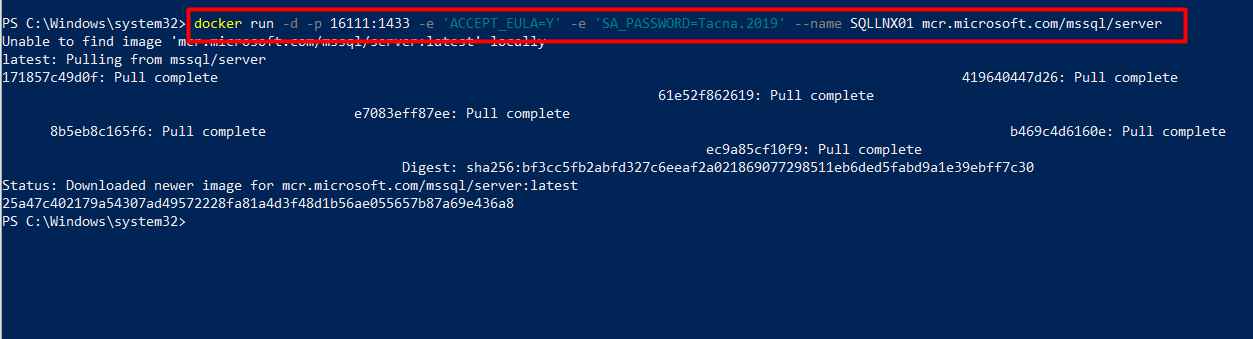
\includegraphics[width=15cm]{./images/1} 
	\end{center}

\textbf{2. Nos conectamos con usuario: sa y clave: Tacna.2020 
}

    \begin{center}
		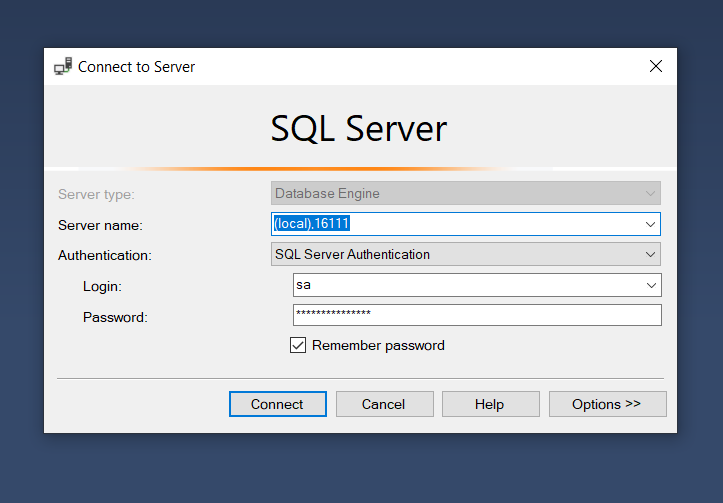
\includegraphics[width=15cm]{./images/2} 
	\end{center}
  \newpage
\textbf{3. Restauramos la base de datos}

    \begin{center}
		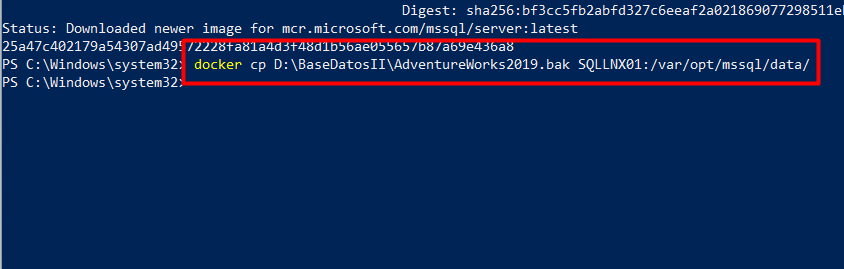
\includegraphics[width=15cm]{./images/3} 
	\end{center}
	
    \begin{center}
		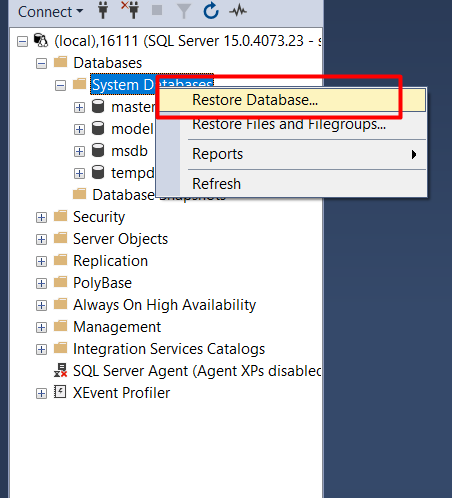
\includegraphics[width=15cm]{./images/4} 
	\end{center}
	
    \begin{center}
		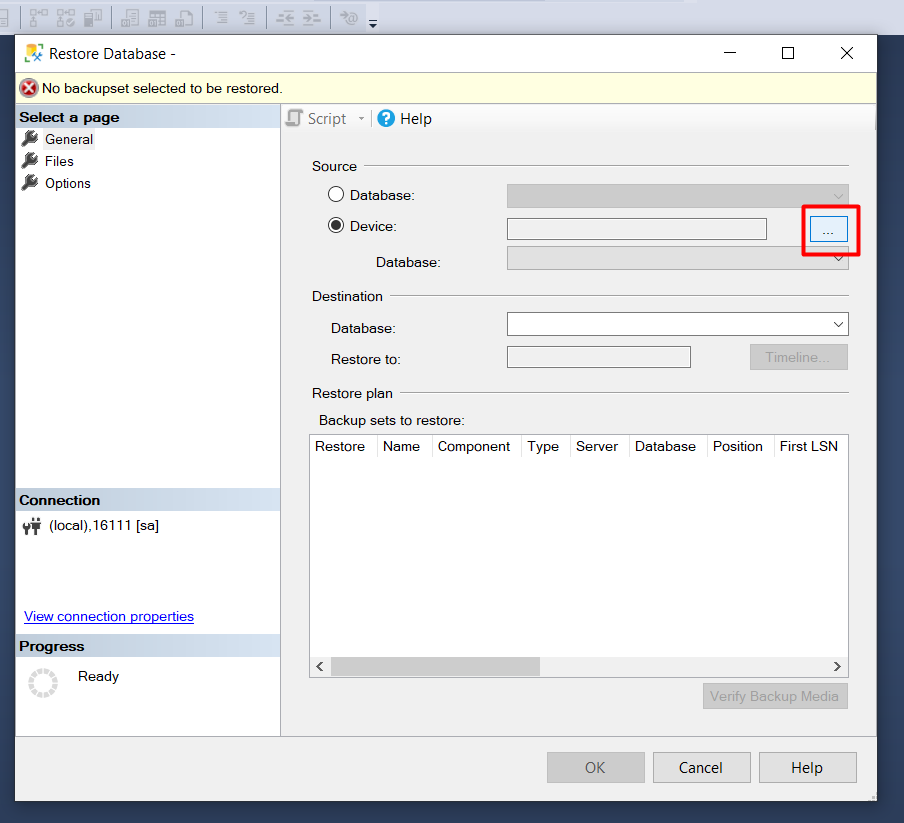
\includegraphics[width=15cm]{./images/5} 
	\end{center}
	
    \begin{center}
		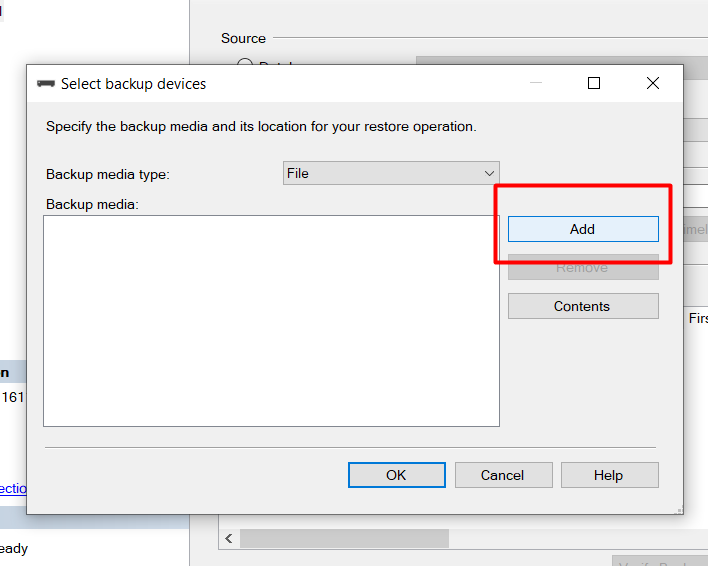
\includegraphics[width=15cm]{./images/6} 
	\end{center}

    \begin{center}
		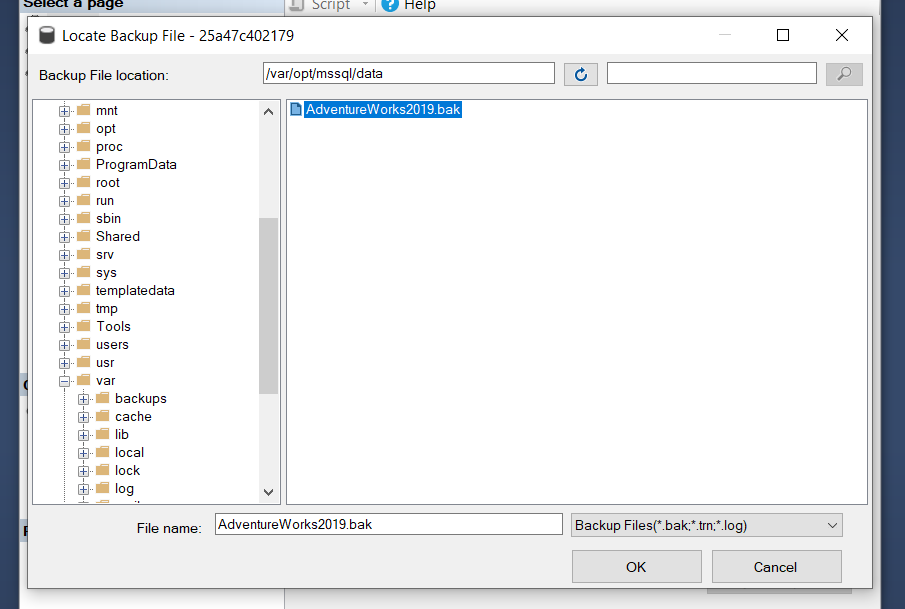
\includegraphics[width=15cm]{./images/7} 
	\end{center}
\newpage
\textbf{4. Abrir la base de datos AdventureWorks.}

    \begin{center}
		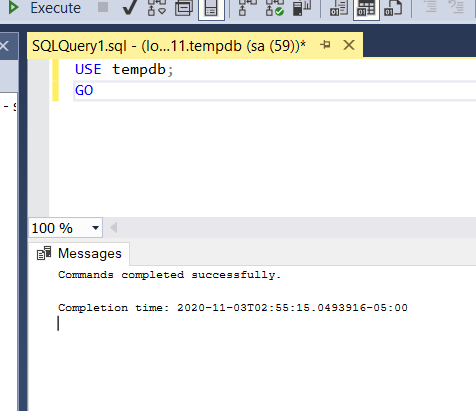
\includegraphics[width=15cm]{./images/11} 
	\end{center}
	

\newpage
\textbf{5.  Consultar las estadisticas físicas de los indices. En la siguiente consulta los tres parametros NULL, son el objeto, el indices y la partición. Por eso se muestran todos los indices.}

   \begin{center}
		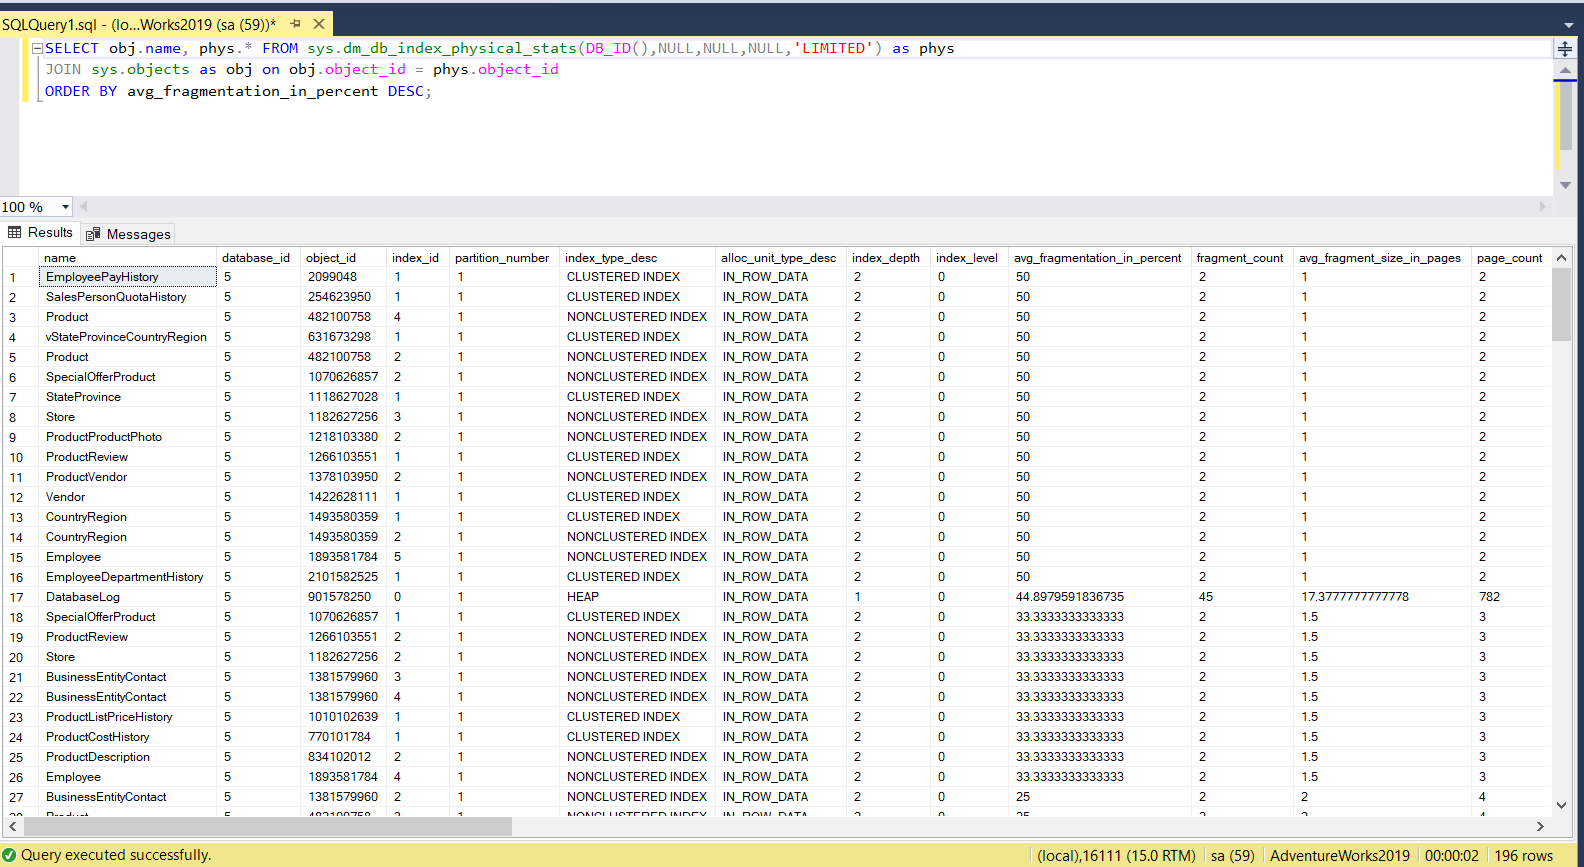
\includegraphics[width=15cm]{./images/8} 
	\end{center}

\textbf{Notas el porcentaje promedio de fragmentación avg_fragmentation_in_percent}

\newpage
\textbf{6. Asimismo hay opciones en el nivel de detalle devuelto. la siguiente opción es SAMPLED.}

    \begin{center}
		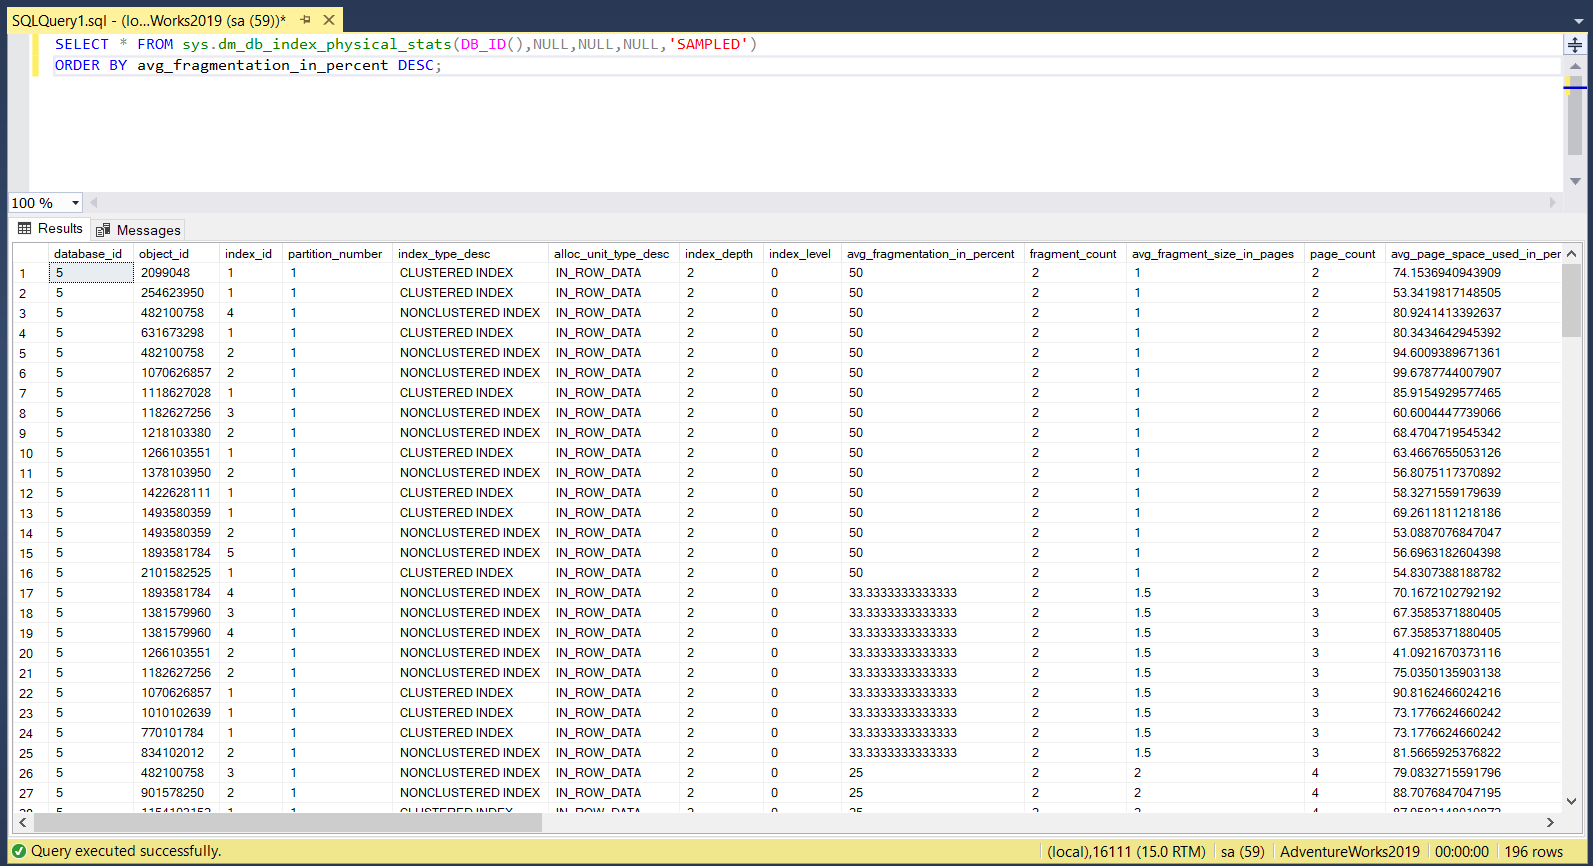
\includegraphics[width=15cm]{./images/9} 
	\end{center}
	
	\newpage
\textbf{7. La opción final es DETAILED. Utilizar con cuidado pues puede demorar la consulta en la BD.}

    \begin{center}
		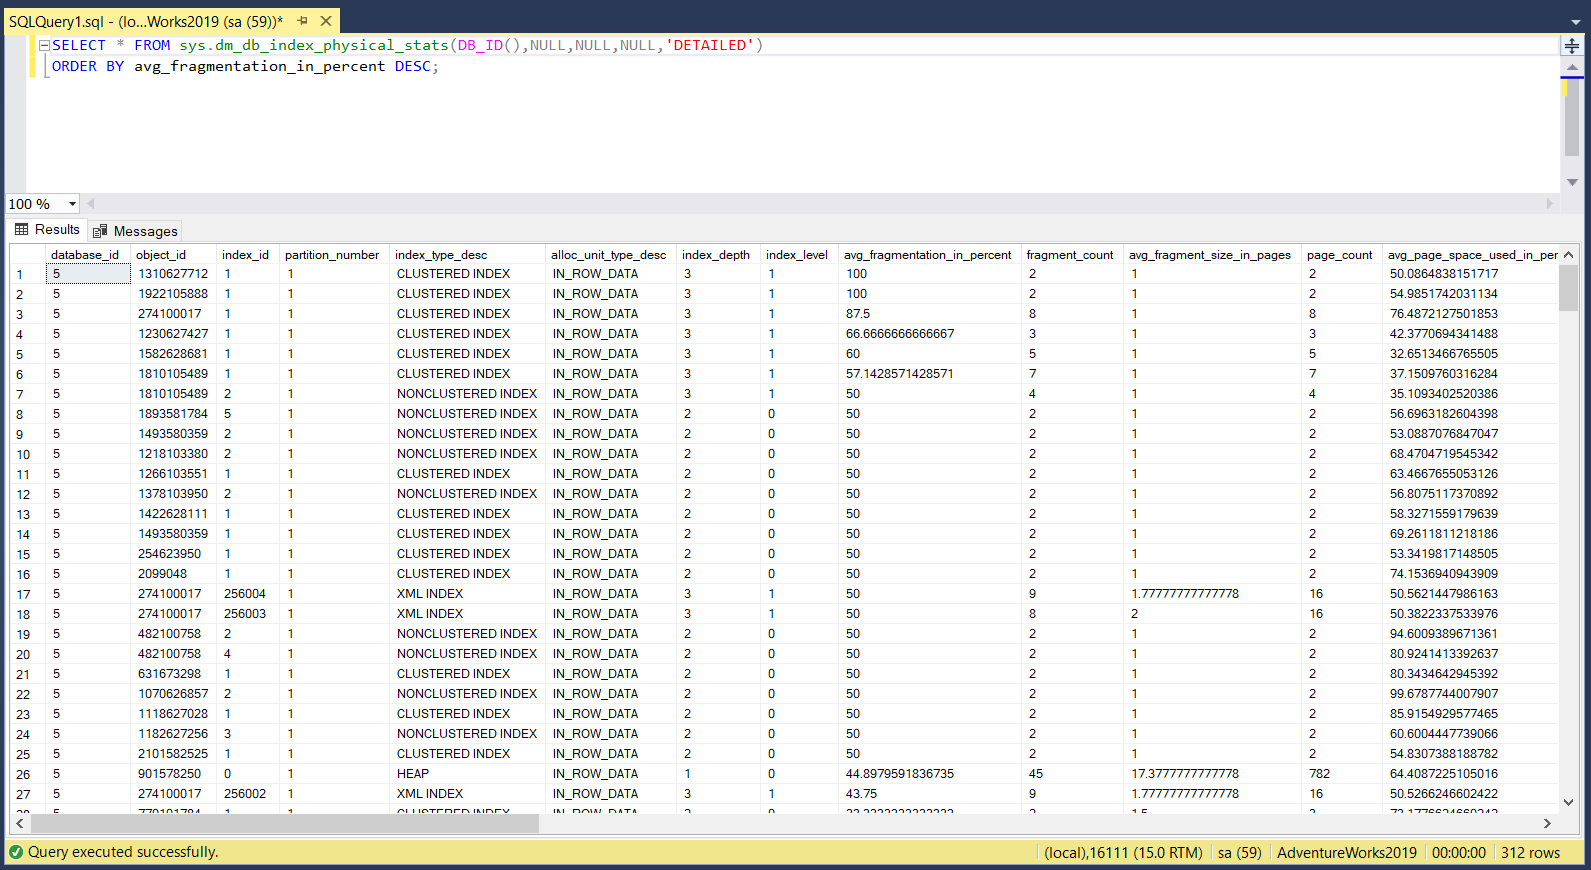
\includegraphics[width=15cm]{./images/10} 
	\end{center}
	\newpage
\textbf{8. Utilizar la base de datos TempDB.}

    \begin{center}
		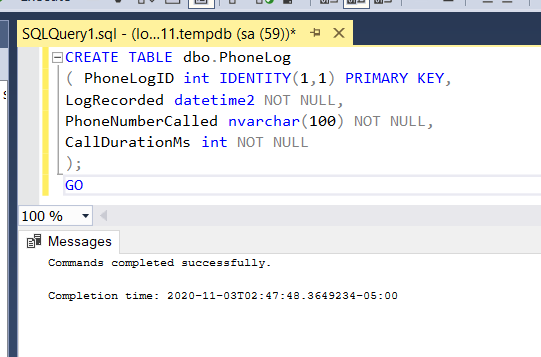
\includegraphics[width=15cm]{./images/12} 
	\end{center}

\textbf{9. Crear una tabla con una llave primaria especificada.}

    \begin{center}
		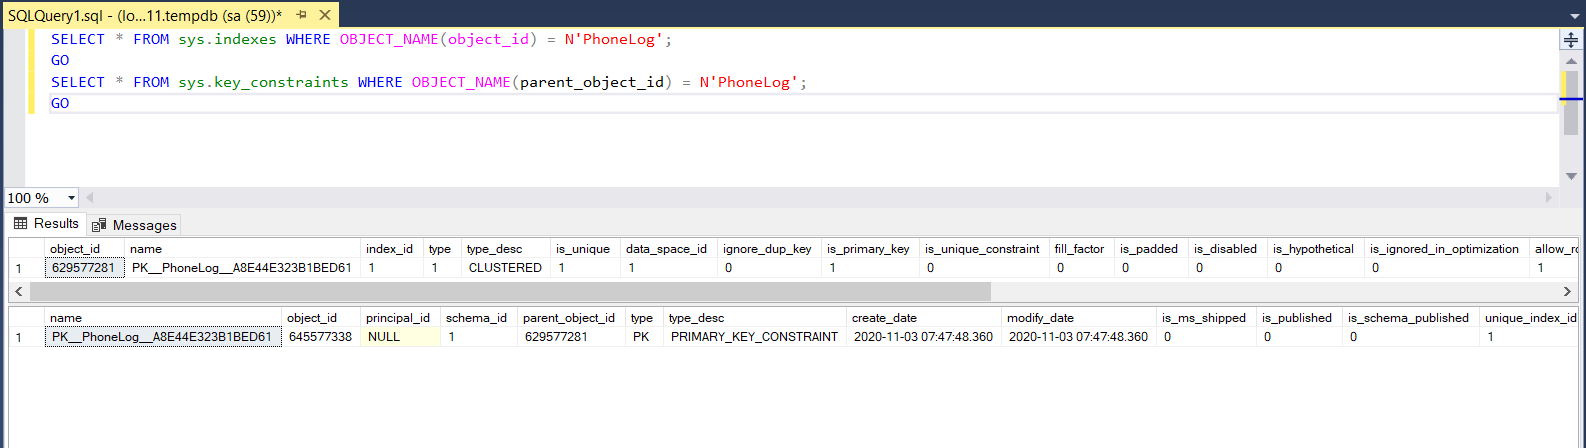
\includegraphics[width=15cm]{./images/13} 
	\end{center}

\newpage
\textbf{10. Consultar sys.indexes para ver la estructura. En el Studio Management se puede utilizar la opción Databases, System Databases, tempdb, Tables, dbo.PhoneLog e Indexes. Show that even though no clustered index was specified, one was created automatically.}

    \begin{center}
		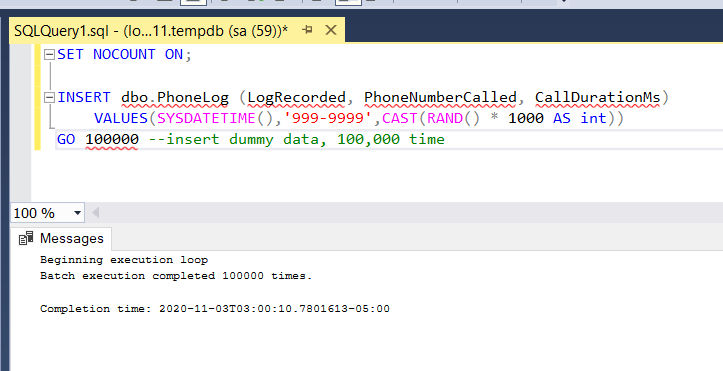
\includegraphics[width=15cm]{./images/14} 
	\end{center}


\textbf{11.  Insertar algunos datos en la tabla.}

    \begin{center}
		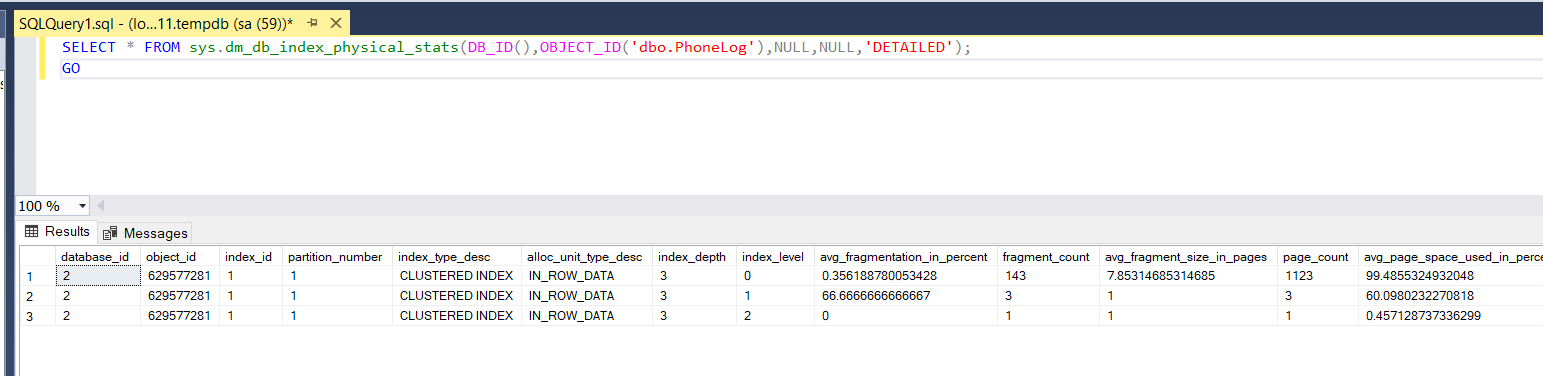
\includegraphics[width=15cm]{./images/15} 
	\end{center}

\newpage
\textbf{12. Revisar el nivel de fragmentación a través de la vista sys.dm_db_index_physical_stats.}

    \begin{center}
		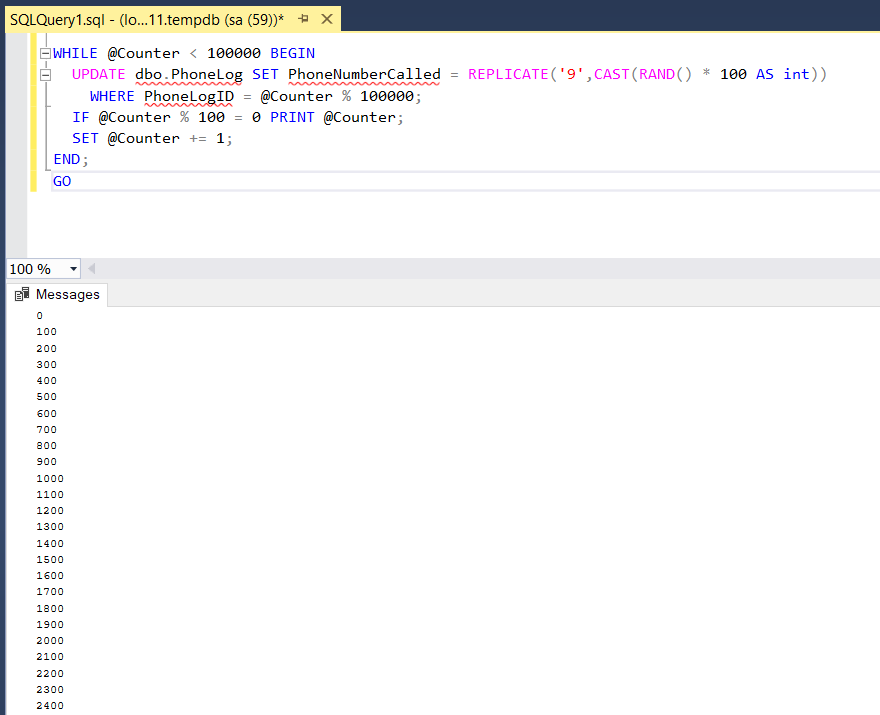
\includegraphics[width=15cm]{./images/16} 
	\end{center}


\textbf{13. Verificar el porcentaje promedio de fragmentación (avg_fragmentation_in_percent y porcentaje promedio de espacio de paginas utilizado (avg_page_space_used_in_percent).}

    \begin{center}
		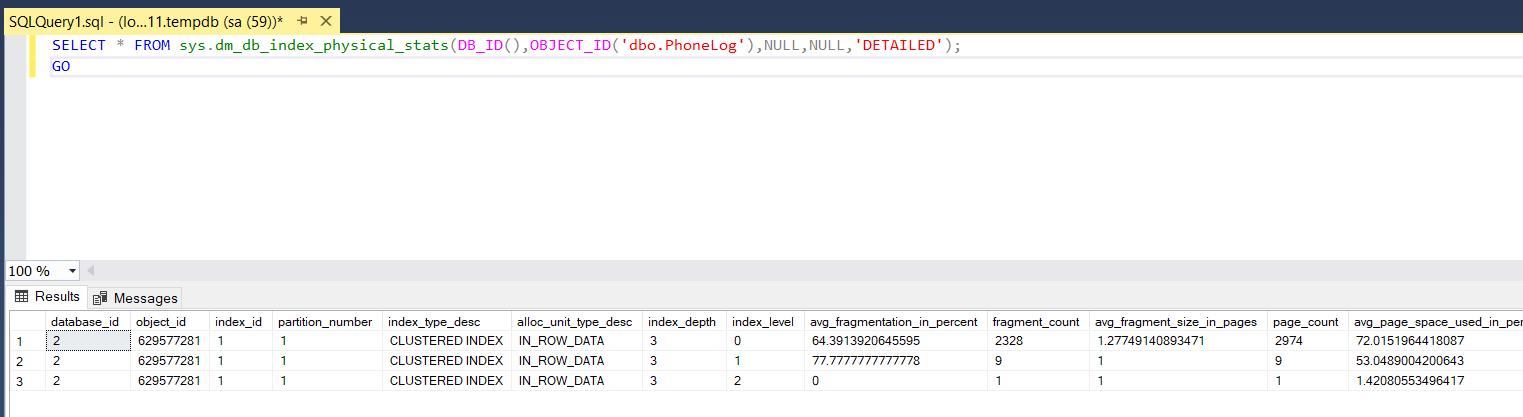
\includegraphics[width=15cm]{./images/17} 
	\end{center}

\textbf{Modificar los datos en la tabla - esto incrementará los datos y ocasionará fragmentación de pagina. Apreciar cuan rapido este comando se ejecuta..}


\textbf{14. Revisar el nivel de fragmentación a través de la vista sys.dm_db_index_physical_stats. Verificar el porcentaje promedio de fragmentación (avg_fragmentation_in_percent y porcentaje promedio de espacio de paginas utilizado (avg_page_space_used_in_percent)}

    \begin{center}
		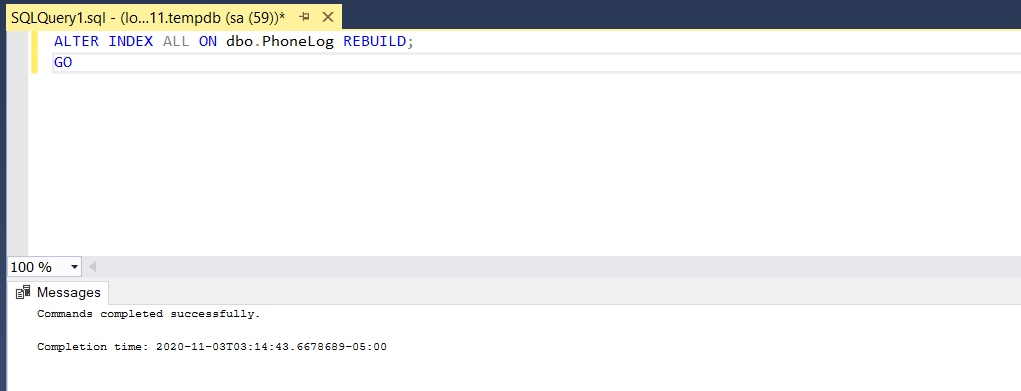
\includegraphics[width=15cm]{./images/18} 
	\end{center}

\textbf{15. Reconstruir la tabla y sus indices.}

    \begin{center}
		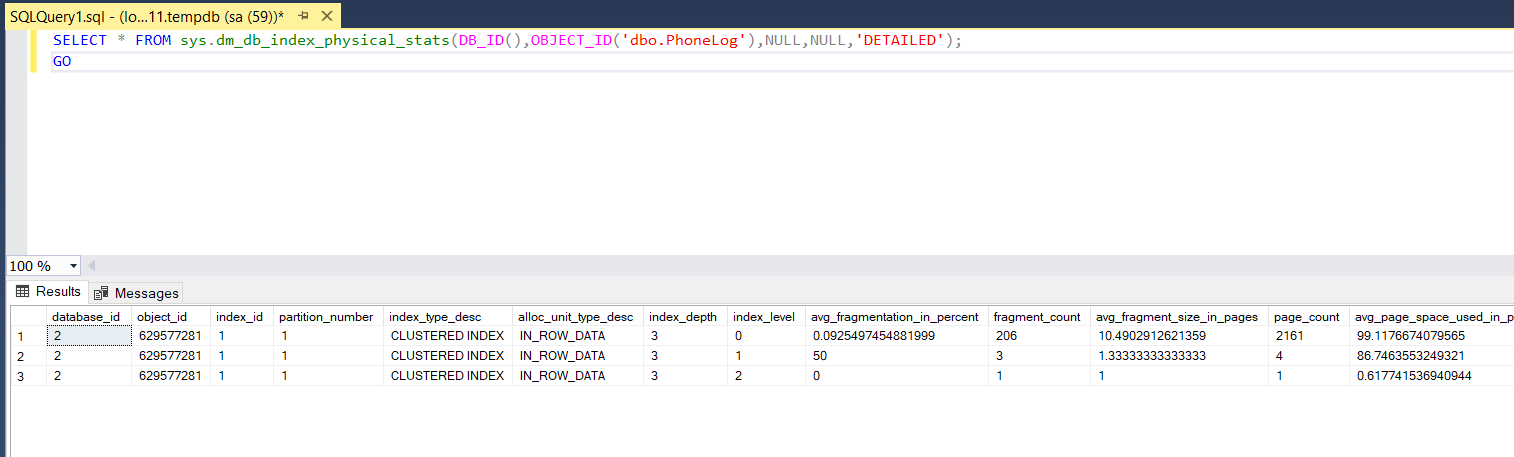
\includegraphics[width=15cm]{./images/19} 
	\end{center}
	\newpage
\textbf{16. Revisar el nivel de fragmentación a través de la vista sys.dm_db_index_physical_stats. Verificar el porcentaje promedio de fragmentación (avg_fragmentation_in_percent y porcentaje promedio de espacio de paginas utilizado (avg_page_space_used_in_percent).}

    \begin{center}
		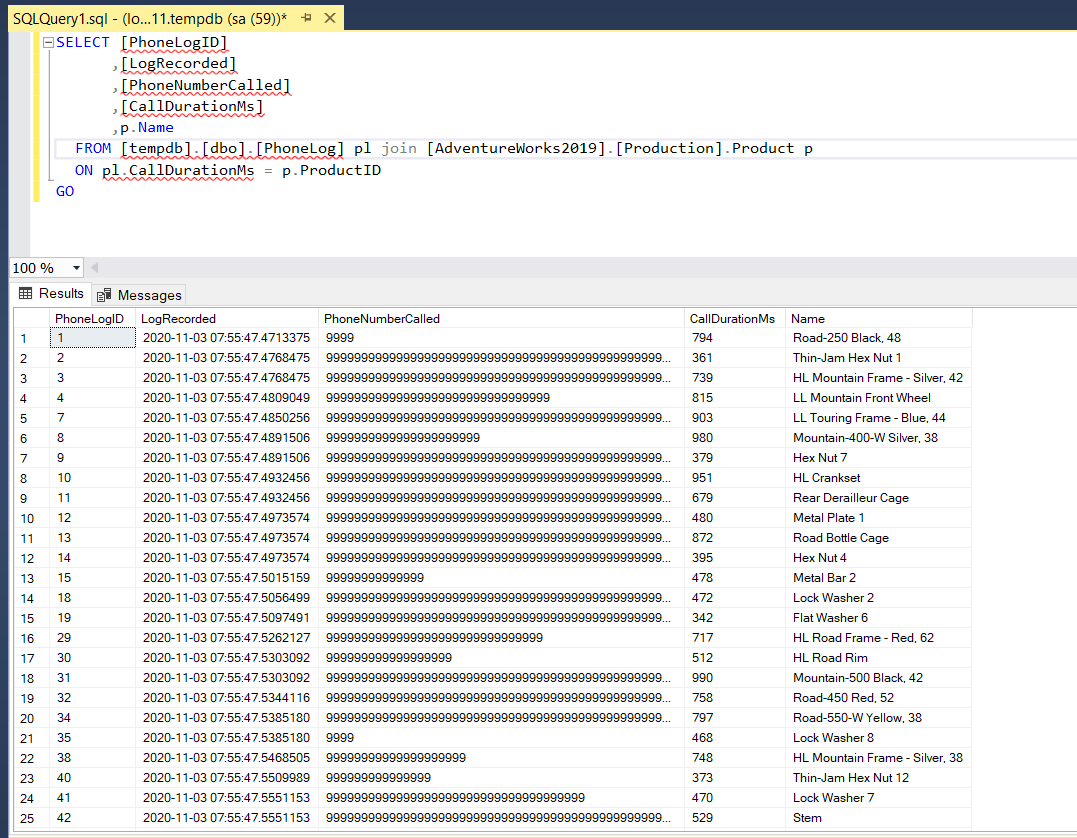
\includegraphics[width=15cm]{./images/20} 
	\end{center}
	\newpage
\textbf{17. Ejecutar una consulta mostrando el plan de ejecución.}

    \begin{center}
		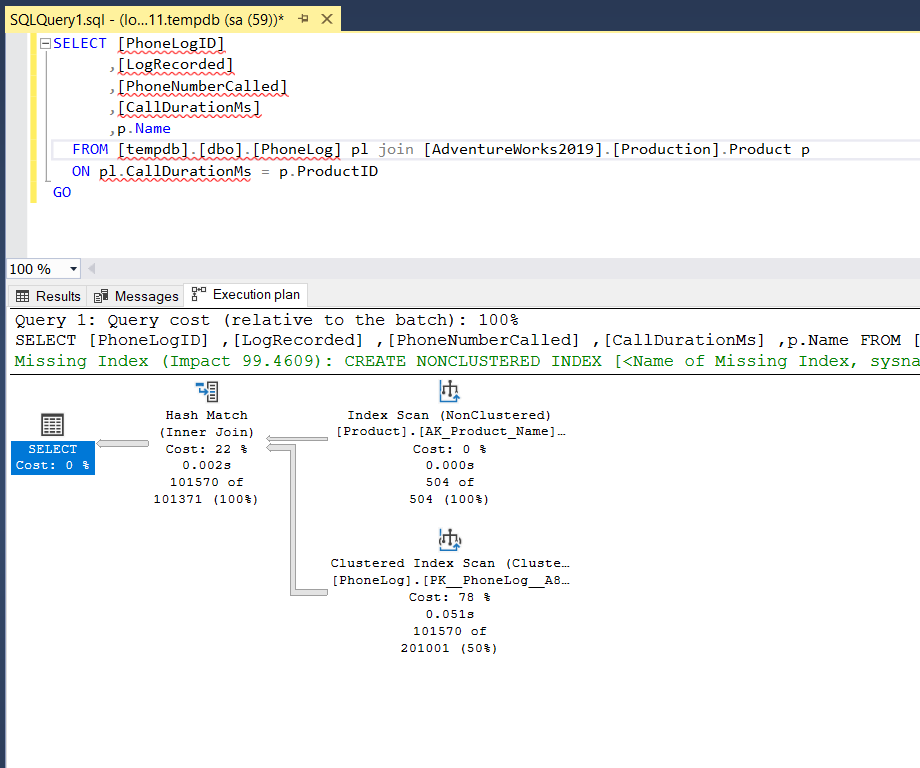
\includegraphics[width=15cm]{./images/21} 
	\end{center}
	\newpage
\textbf{18. Crear un índice de cobertura, apuntando a las columnas incluidas.}

    \begin{center}
		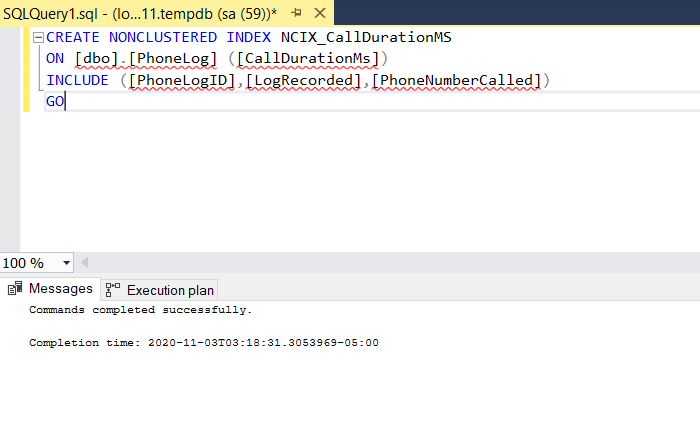
\includegraphics[width=15cm]{./images/22} 
	\end{center}
	\newpage
\textbf{19. Ejecutar una consulta mostrando el plan de ejecución. Ahora utiliza el nuevo indice.}

    \begin{center}
		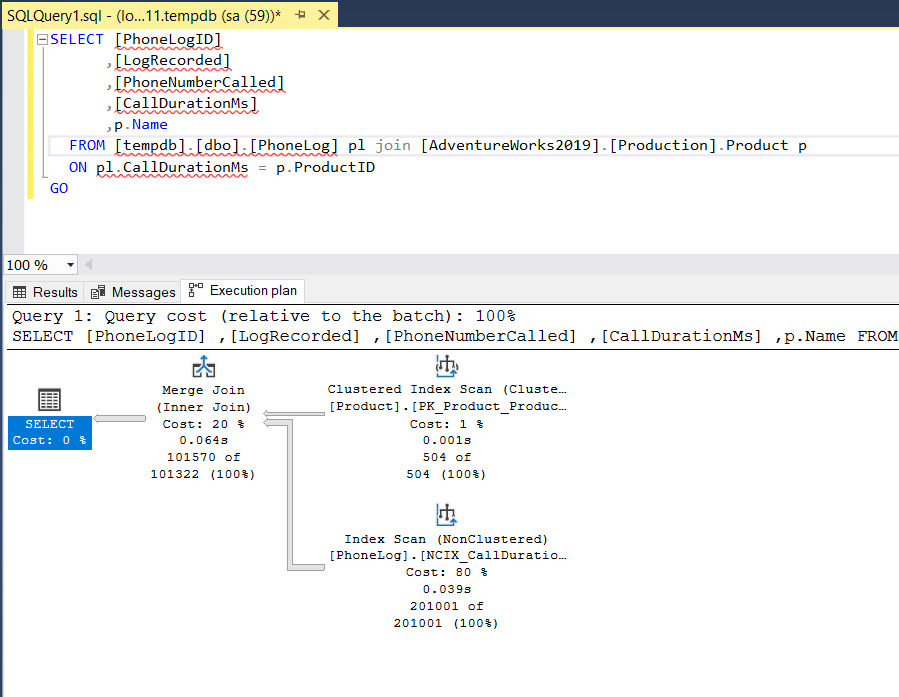
\includegraphics[width=15cm]{./images/23} 
	\end{center}
\newpage
\textbf{20. Eliminar la tabla.}

    \begin{center}
		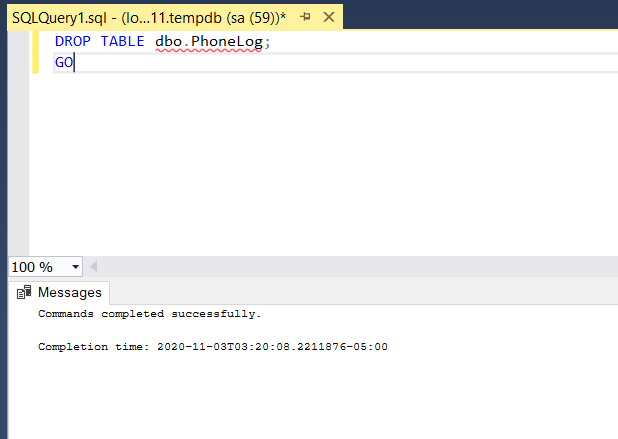
\includegraphics[width=15cm]{./images/24} 
	\end{center}
\newpage
\textbf{21. Seleccionar nuevamente la base de datos AdventureWorks. Revisar las estadisticas de la llave primaria de la tabla Sales.SalesOrderDetail.}

    \begin{center}
		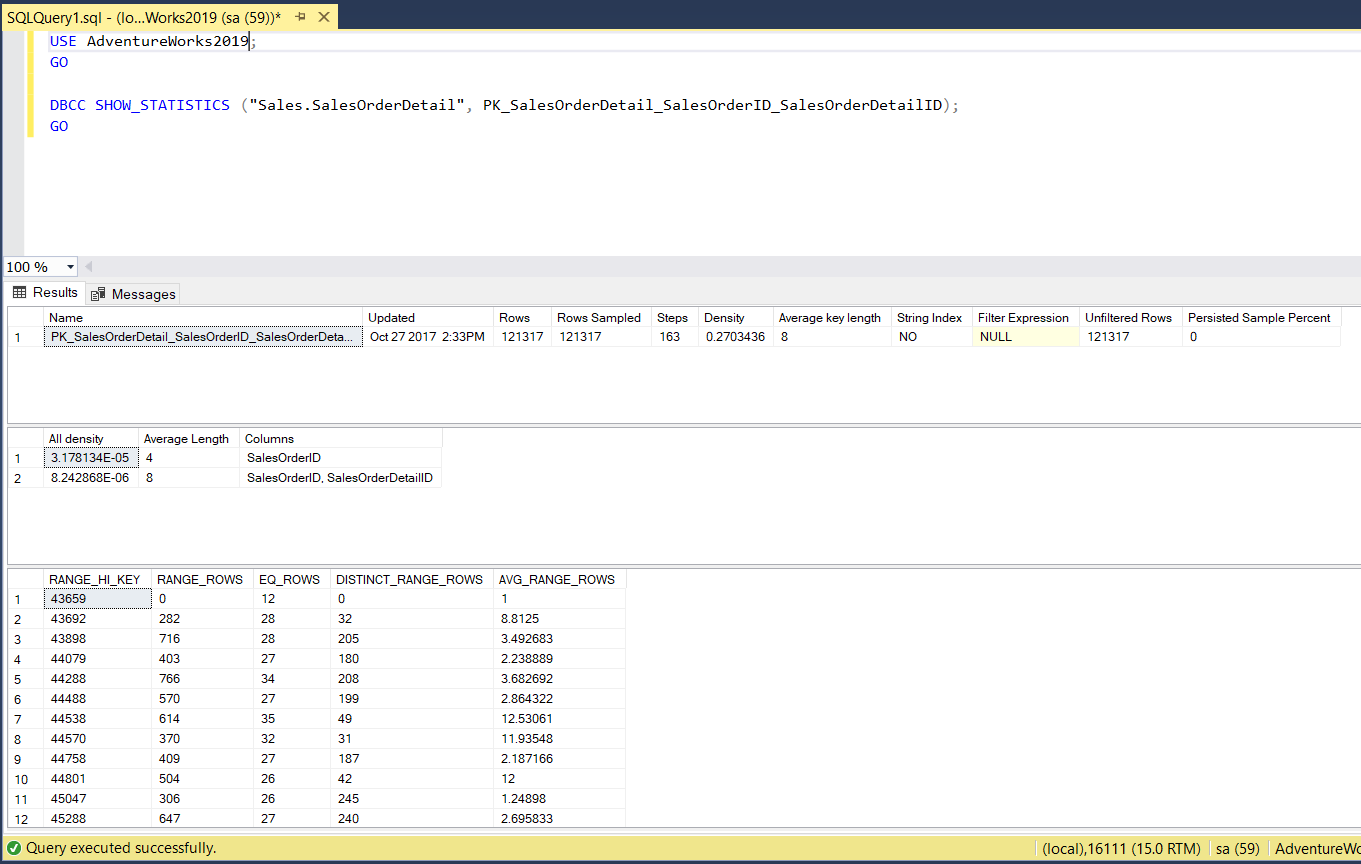
\includegraphics[width=15cm]{./images/25} 
	\end{center}
\newpage
\textbf{22. Ejecutar el script siguiente y verificar la estadistica actualiza utilizando el plan de ejecuión.}

    \begin{center}
		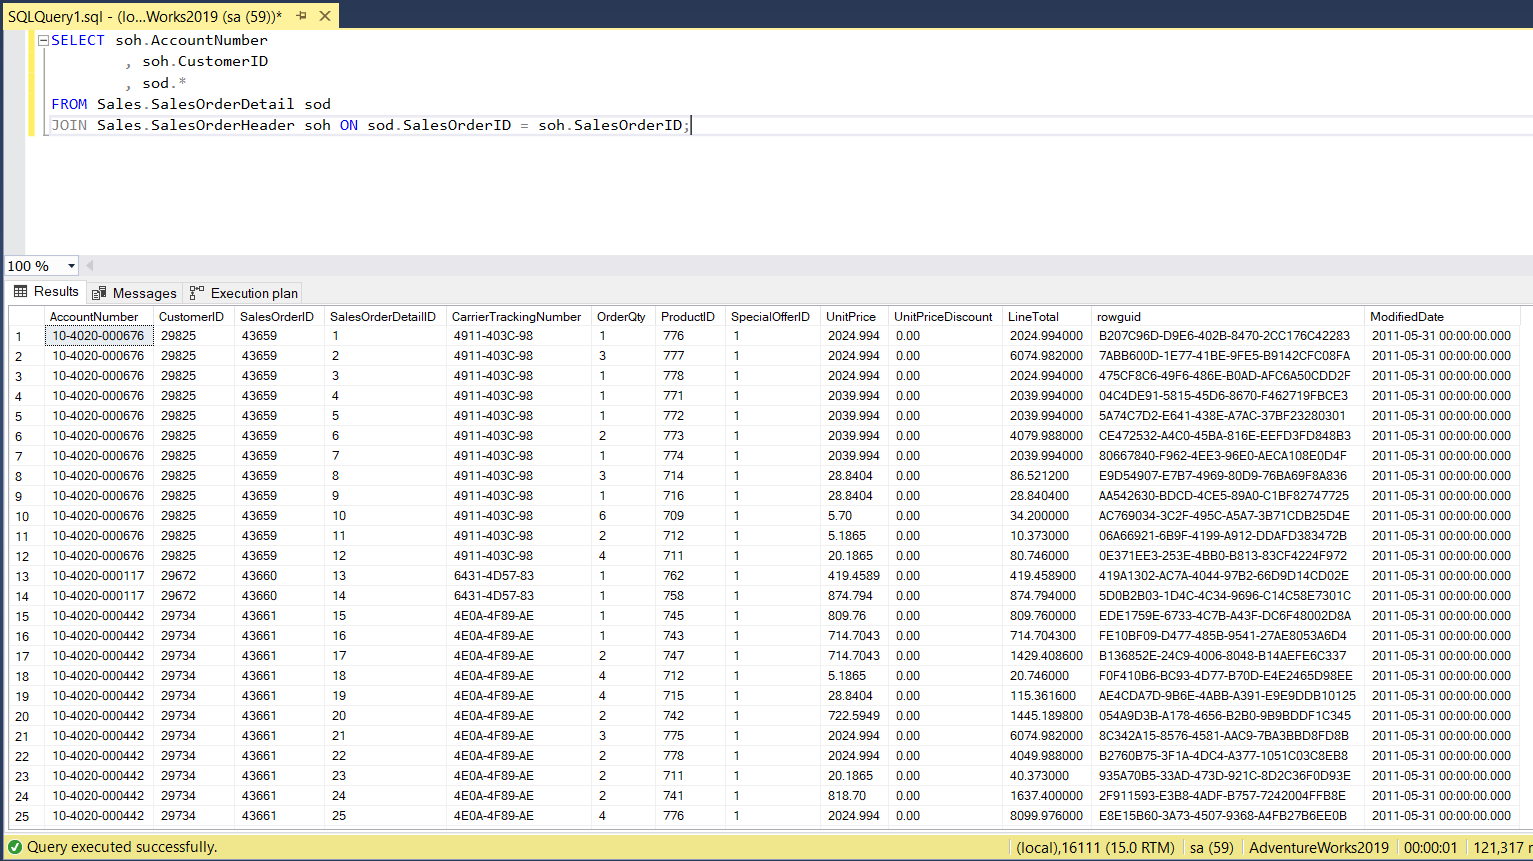
\includegraphics[width=15cm]{./images/26} 
	\end{center}

   
\end{document}
